Nesta seção, são apresentados os materiais e métodos utilizados no desenvolvimento do sistema. Isso inclui as ferramentas e tecnologias empregadas, a arquitetura do sistema e as integrações realizadas.

\section{Descrição da área de estudo}
O sistema em questão foi implementado no Instituto Federal de Minas Gerais (IFMG), \textit{campus} Bambuí, especificamente no laboratório de elétrica. Esse local foi escolhido por possuir uma infraestrutura adequada para o teste de sensores e equipamentos necessários para a captura e transmissão de dados. A escolha do laboratório também se deve à disponibilidade de supervisão técnica e apoio logístico para a instalação e validação dos equipamentos.

\section{Sistema de monitoramento meteorológico}
O sistema desenvolvido utiliza uma série de sensores para monitorar em tempo real diferentes parâmetros meteorológicos. Os componentes do sistema incluem:

\begin{itemize}
\item Anemômetro (Figura \ref{figura:anemometro});
\item Sensor de temperatura e umidade do ar DHT22 (Figura \ref{figura:sensor_dht22});
\item Sensor de pressão barométrica BMP280 (Figura \ref{figura:sensor_bmp280});
\item Sensor de umidade do solo LM393 (Figura \ref{figura:sensor_lm393});
\item Sensor de luminosidade BH1750 (Figura \ref{figura:sensor_bh1750});
\item Microcontrolador ESP32 (Figura \ref{figura:esp32});
\item \textit{Jumpers} e cabos (Figura \ref{figura:jumpers}).
\end{itemize}

Esses componentes foram integrados em um sistema cyber-físico que publica as leituras individuais de cada sensor em um \textit{broker}. Nesse trabalho optou-se pelo \textit{EMQX}, uma plaforma de código aberto para MQTT de alta performance \parencite{EMQX}.

Nele as mensagens são distribuídas em tópicos de forma persistente e segura, usando protocolos de comunicação (MQTT) e criptografia (TLS). Isso garante a integridade e a confidencialidade dos dados coletados, além do acesso remoto e em tempo real às leituras. Este acesso é feito através da conexão entre o \textit{broker} e o \textit{backend} do sistema, que se inscreve nos tópicos de interesse para receber os dados. Também é feita uma segunda instância de armazenamento em um banco de dados relacional (\textit{MySQL}) para consultas de interesse.

\section{Ferramentas e tecnologias utilizadas}
As ferramentas e tecnologias empregadas para o desenvolvimento do sistema incluem:

\begin{itemize}
\item \textit{Node.js} como ambiente de execução do \textit{backend};
\item \textit{React} como biblioteca de desenvolvimento de interfaces para o \textit{frontend};
\item \textit{Nest.js} como \textit{framework} para o \textit{backend};
\item \textit{Vitest} como \textit{framework} de testes;
\item \textit{Prisma} como mapeador objeto-relacional (ORM);
\item \textit{Shadcn/ui} como biblioteca de componentes para o \textit{frontend};
\item \textit{Tailwind CSS} como \textit{framework} de estilização;
\item MQTT como protocolo de comunicação entre os sensores e o \textit{backend};
\item HTTP como protocolo de comunicação entre o \textit{backend} e o \textit{frontend};
\item \textit{Figma} para prototipagem de interfaces gráficas;
\item \textit{MySQL} como banco de dados relacional;
\item Visual Studio Code para desenvolvimento web;
\item Arduino IDE para desenvolvimento embarcado;
\item \textit{Fritzing} para prototipagem de circuitos;
\item \textit{EasyEDA} para desenho de placas de circuito impresso (PCB).
\end{itemize}

Essas tecnologias foram selecionadas por sua capacidade de suportar um sistema de monitoramento robusto e eficiente, garantindo a precisão e a escalabilidade necessárias para o monitoramento em tempo real.

\section{Métodos de análise de dados}
Os dados meteorológicos são processados e analisados utilizando as tecnologias mencionadas. A análise é realizada de forma contínua para apresentar medições e cálculos estimativos de ETo e ETc locais. Esse método de análise permite a interpretação e avaliação dos dados de forma rápida, além de gerar relatórios periódicos para a tomada de decisões.

\section{Estimativa da evapotranspiração}

O cálculo da ETo e da ETc é usada para o monitoramento hídrico em tempo real e é realizado com base nas leituras dos sensores. Foram usadas as equações da FAO-56 como modelagem referencial. Cada leitura dos sensores contribui diretamente para o cálculo dessas variáveis ou é convertida de forma a ser utilizada na equação.

\subsection{Variáveis meteorológicas e sua obtenção}

As variáveis meteorológicas utilizadas no cálculo da evapotranspiração são obtidas da seguinte forma:
\begin{itemize}
    \item A temperatura do ar (\(T\)) é medida diretamente do sensor DHT22, que fornece a temperatura em graus Celsius;
    
    \item A umidade relativa (\(RH\)) também é medida pelo sensor DHT22, em percentual;
    
    \item A pressão atmosférica (\(P\)) é obtida do sensor BMP280, em hPa;

    \item A velocidade do vento (\(u_2\)) é medida pelo anemômetro, em m/s.
\end{itemize}

As demais variáveis são estimadas a partir de cálculos intermediários, obtidos, com excessão da radiação líquida, da obra de \textcite{thermodynamic_fermi}:
\begin{itemize}
    \item A radiação líquida (\(R_n\)) é estimada a partir das leituras do sensor de luminosidade BH1750, que mede a intensidade luminosa em lux. \textcite{Michael_2020} apresenta a conversão de lux para radiação líquida em MJ/m²/dia, dada pela equação:
    
    \[ R_n = \frac{Lux}{100000} \times 0.0036 \times 0.0864 \times 1000 \]
    
    \item A variação da pressão de saturação (\(\Delta\)) é calculada com a equação:
    \[
    \Delta = \frac{4098 \cdot (0.6108 \cdot e^{\frac{17.27 \cdot T}{T + 237.3}})}{(T + 237.3)^2}
    \]
    
    \item A pressão de saturação (\(e_s\)) é calculada usando:
    \[
    e_s = 0.6108 \cdot e^{\frac{17.27 \cdot T}{T + 237.3}}
    \]
    
    \item A pressão de vapor atual (\(e_a\)) é obtida com:
    \[
    e_a = \frac{RH}{100} \cdot e_s
    \]
    
    \item O fluxo de calor do solo (\(G\)) pode ser assumido como nulo, ou seja, considera-se \(G = 0\);
    
    \item A constante psicrométrica (\(\gamma\)) é dada por:
    \[
    \gamma = \frac{0.665 \times 10^{-3} \times P}{\lambda}
    \]
    onde \(\lambda\) é o calor de vaporização da água, aproximadamente 2.45 MJ/kg.
\end{itemize}

\section{Desenvolvimento da aplicação}
Nessa subsessão, são apresentados os detalhes do desenvolvimento da aplicação, incluindo a arquitetura do sistema e os métodos de prototipagem utilizados.

\subsection{Padrões arquiteturais práticas utilizadas}

No desenvolvimento do sistema, foram adotados padrões arquiteturais para garantir a modularidade, escalabilidade e manutenção do código. A arquitetura foi baseada nos princípios de \textit{Domain-Driven Design} (DDD) e nos cinco princípios SOLID \parencite{ddd_eric2004}.

O DDD foi escolhido como base para a estruturação do sistema devido à sua capacidade de refletir com precisão a complexidade do domínio meteorológico no código. A aplicação foi dividida em camadas como \textit{domain}, \textit{application}, \textit{infrastructure}, e \textit{interfaces}, onde cada uma possui responsabilidades bem definidas. Isso facilita a evolução e adaptação do sistema a novos requisitos.

Os princípios SOLID foram aplicados para garantir um código coeso, desacoplado e extensível. Especificamente:
\begin{itemize}
    \item O princípio da responsabilidade única (SRP) foi adotado para garantir que cada classe ou módulo tenha uma única responsabilidade, facilitando a manutenção e evolução do código;
    \item O princípio aberto/fechado (OCP) assegurou que os componentes do sistema fossem abertos para extensão, mas fechados para modificação, permitindo a adição de novas funcionalidades sem alterar o código existente;
    \item O princípio da substituição de Liskov (LSP) foi utilizado para garantir que as classes derivadas pudessem substituir suas classes base sem alterar o comportamento do sistema;
    \item O princípio da segregação de interfaces (ISP) assegurou que as interfaces fossem específicas para cada tipo de cliente, evitando a implementação de métodos desnecessários;
    \item O princípio da inversão de dependência (DIP) foi seguido para garantir que módulos de alto nível não dependessem de módulos de baixo nível, mas sim de abstrações, promovendo o desacoplamento do código.
\end{itemize}

Essas práticas resultaram em um código mais limpo, testável e resiliente, capaz de suportar a evolução contínua do sistema sem comprometer sua integridade.

\subsection{Ciclo de desenvolvimento do software}

O ciclo de desenvolvimento do \textit{software} envolveu tanto a parte \textit{web} quanto a embarcada, seguindo uma abordagem iterativa e incremental, utilizando \textit{Git Workflow} como estratégia principal de controle de versões \parencite{pro_git}.

Para o desenvolvimento \textit{web}, o fluxo começou com a definição dos requisitos e a modelagem do domínio, seguida pela implementação das funcionalidades em \textit{branches} específicas, alinhadas com as funcionalidades do sistema. Cada \textit{feature branch} era integrada à \textit{branch develop} após a aprovação em revisões de código e a passagem pelos testes automatizados, garantindo a qualidade e a integração contínua do código. O \textit{Git Workflow} utilizado incluía a criação de \textit{feature branches}, \textit{hotfix branches}, e \textit{release branches}, de acordo com o estado de desenvolvimento e manutenção do sistema.

Para o desenvolvimento embarcado, foram utilizados ciclos mais curtos devido à necessidade de validação rápida dos sensores e componentes físicos. Cada ciclo incluía a configuração do \textit{hardware}, programação do \textit{firmware} no ESP32 utilizando a Arduino IDE, e testes físicos para validação dos dados coletados. As versões do código embarcado eram gerenciadas em um repositório \textit{Git} separado, seguindo uma estrutura similar à usada para o desenvolvimento \textit{web}, mas adaptada para as necessidades específicas do desenvolvimento embarcado, incluindo a verificação de integrações entre sensores e o envio dos dados ao EMQX.

A sinergia entre essas duas frentes de desenvolvimento foi usada para garantir que o sistema operasse de forma coesa e integrada, desde a captura dos dados até a sua visualização na interface \textit{web}.

\subsection{Prototipagem e distribuição dos componentes}

A prototipagem do sistema foi uma etapa importante para garantir que os componentes de \textit{hardware} e \textit{software} funcionassem harmoniosamente. O processo começou com a criação de protótipos de baixa fidelidade, utilizando o \textit{Fritzing} para o design dos circuitos e a prototipagem das interações entre os sensores e o microcontrolador ESP32.

O desenvolvimento do protótipo envolveu a montagem dos sensores em uma \textit{breadboard}, permitindo ajustes rápidos e trocas de componentes conforme necessário. O \textit{layout} dos componentes foi projetado no \textit{EasyEDA} de forma a otimizar a coleta de dados, minimizando interferências e garantindo a precisão das medições. Após a validação do protótipo inicial, os componentes foram migrados para uma montagem mais permanente, utilizando uma PCB e cabos soldados, garantindo maior durabilidade e estabilidade nas leituras.

Para a prototipagem do \textit{software}, foram utilizados \textit{mockups} e \textit{wireframes} para definir as interfaces e fluxos de usuário. Ferramentas como \textit{Figma} foram empregadas para criar protótipos de alta fidelidade das telas, que serviram de guia para o desenvolvimento do frontend em \textit{React}. A distribuição dos componentes de \textit{software} seguiu o princípio de modularidade, permitindo que cada módulo fosse desenvolvido e testado isoladamente antes de ser integrado ao sistema principal.

A metodologia adotada permitiu uma transição suave do protótipo para a implementação final, garantindo que todos os componentes do sistema fossem adequadamente validados e integrados antes da implantação no laboratório.

\section{Classificação da pesquisa}

A pesquisa realizada no desenvolvimento do sistema de monitoramento meteorológico pode ser classificada segundo os seguintes critérios: quanto aos objetivos, à natureza, aos procedimentos técnicos, e à abordagem do problema.

\subsection{Quanto aos objetivos}

De acordo com os objetivos, esta pesquisa é classificada como descritiva e exploratória. 

A pesquisa é descritiva porque visa descrever as características dos fenômenos meteorológicos monitorados pelos sensores, bem como o comportamento do sistema de monitoramento implementado. O foco está em detalhar como as variáveis meteorológicas, como temperatura, umidade, pressão, velocidade do vento e luminosidade, são capturadas e processadas pelo sistema, além de documentar o desempenho dos componentes de \textit{hardware} e \textit{software} utilizados.

A pesquisa também é exploratória porque busca investigar a aplicabilidade e eficiência de diferentes tecnologias e métodos no monitoramento meteorológico. Isso inclui a experimentação com diversos sensores e técnicas de integração de dados em um contexto específico. O caráter exploratório é acentuado pela busca de soluções tecnológicas que possam ser escaláveis e aplicáveis a diferentes contextos de monitoramento ambiental.

\subsection{Quanto à natureza}

Quanto à natureza, a pesquisa é aplicada. O objetivo principal é o desenvolvimento de uma solução prática para um problema real, neste caso, a necessidade de monitoramento meteorológico em tempo real. O conhecimento gerado é voltado para a aplicação direta no sistema desenvolvido, com o propósito de melhorar a coleta, processamento e análise de dados meteorológicos. A pesquisa aplicada busca, portanto, transformar o conhecimento teórico em soluções práticas e funcionais.

\subsection{Quanto aos procedimentos técnicos}

Em relação aos procedimentos técnicos, a pesquisa é classificada como experimental. Durante o desenvolvimento do sistema, foram realizados testes e experimentos com diferentes componentes \textit{hardware} e \textit{software}, a fim de avaliar seu desempenho e adequação ao monitoramento meteorológico. Esses testes incluíram a validação dos sensores, a integração com o microcontrolador ESP32, e a transmissão de dados através do protocolo MQTT. A pesquisa experimental permitiu ajustes e refinamentos no sistema até alcançar um protótipo funcional e validado.

\subsection{Quanto à abordagem do problema}

Quanto à abordagem do problema, esta pesquisa é quantitativa. O sistema desenvolvido coleta, processa e analisa dados meteorológicos numéricos, que são quantificados e apresentados em relatórios e gráficos. A análise quantitativa é usada para a interpretação dos dados capturados pelos sensores, permitindo a avaliação precisa de variáveis como temperatura, umidade, pressão, e velocidade do vento, além de possibilitar o cálculo de índices climáticos, como a evapotranspiração. A abordagem quantitativa foi escolhida por sua capacidade de fornecer resultados objetivos e mensuráveis, fundamentais para o monitoramento e a tomada de decisão baseada em dados.

\begin{figure}[!htb] \centering
\caption{Anemômetro} \label{figura:anemometro}
\begin{varwidth}{\linewidth}
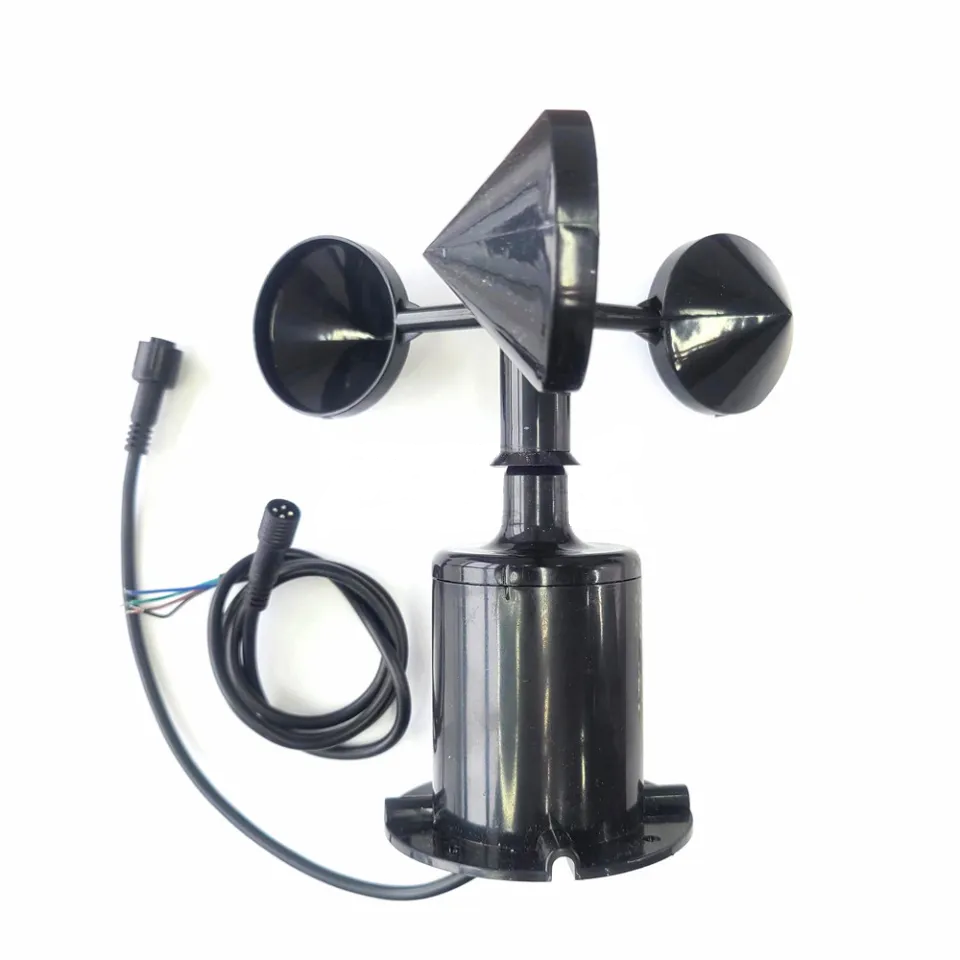
\includegraphics[width=10cm]{figuras/Anemometer-sensor.png}
\fonte{Retirado de \textcite{Eletrogate}.}
\end{varwidth}
\end{figure}

\begin{figure}[!htb] \centering
\caption{Sensor DHT22} \label{figura:sensor_dht22}
\begin{varwidth}{\linewidth}
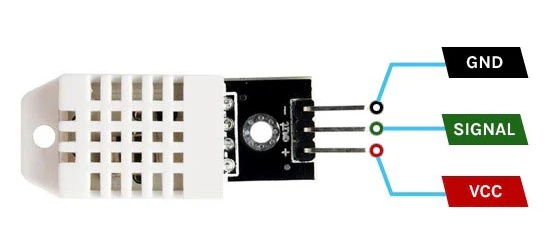
\includegraphics[width=10cm]{figuras/DHT22-sensor.png}
\fonte{Retirado de \textcite{Eletrogate}.}
\end{varwidth}
\end{figure}

\begin{figure}[!htb] \centering
\caption{Sensor BMP280} \label{figura:sensor_bmp280}
\begin{varwidth}{\linewidth}
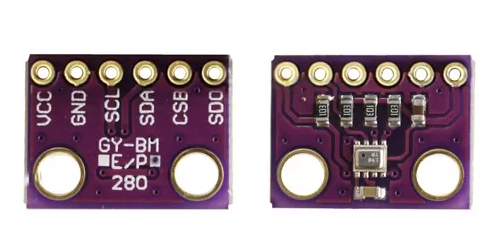
\includegraphics[width=10cm]{figuras/BMP280-sensor.png}
\fonte{Retirado de \textcite{Eletrogate}.}
\end{varwidth}
\end{figure}

\begin{figure}[!htb] \centering
\caption{Sensor LM393} \label{figura:sensor_lm393}
\begin{varwidth}{\linewidth}
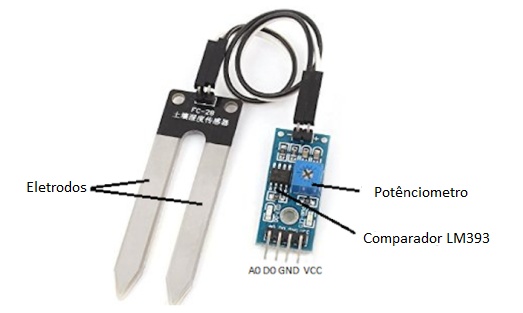
\includegraphics[width=10cm]{figuras/LM393-sensor.png}
\fonte{Retirado de \textcite{Eletrogate}.}
\end{varwidth}
\end{figure}

\begin{figure}[!htb] \centering
\caption{Sensor BH1750} \label{figura:sensor_bh1750}
\begin{varwidth}{\linewidth}
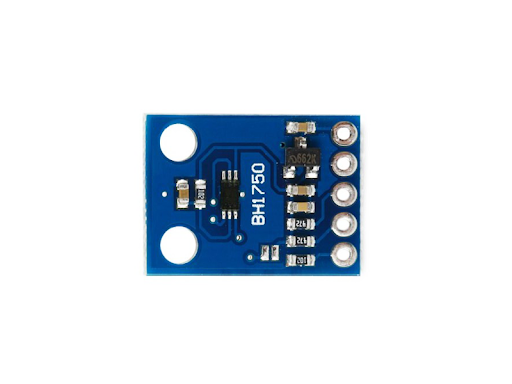
\includegraphics[width=10cm]{figuras/BH1750-sensor.png}
\fonte{Retirado de \textcite{Eletrogate}.}
\end{varwidth}
\end{figure}

\begin{figure}[!htb] \centering
\caption{Microcontrolador ESP32} \label{figura:esp32}
\begin{varwidth}{\linewidth}
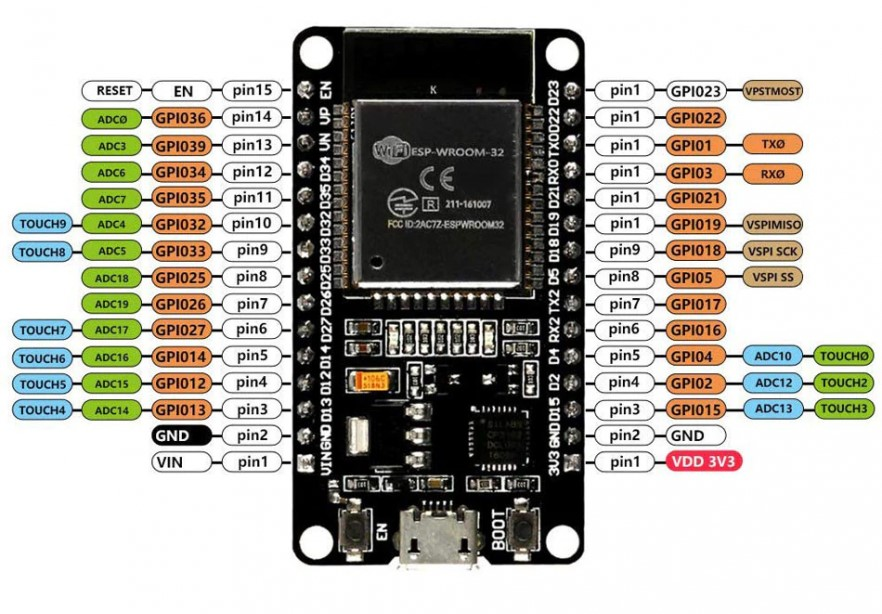
\includegraphics[width=10cm]{figuras/ESP32-micro.jpg}
\fonte{Retirado de \textcite{Eletrogate}.}
\end{varwidth}
\end{figure}

\begin{figure}[!htb] \centering
\caption{\textit{Jumpers}} \label{figura:jumpers}
\begin{varwidth}{\linewidth}
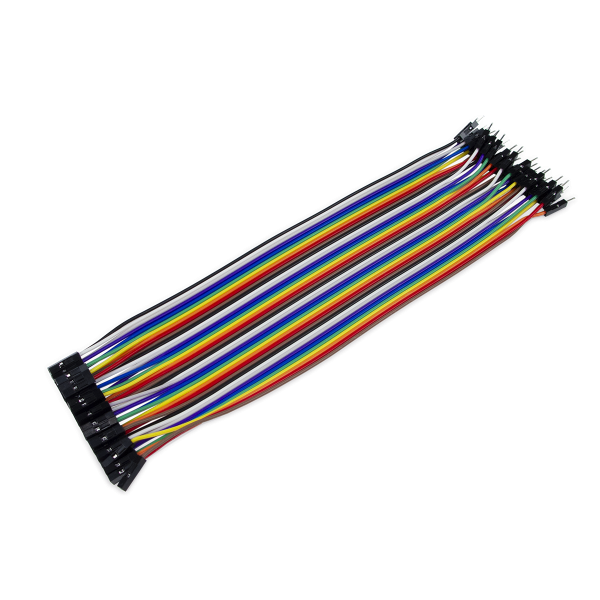
\includegraphics[width=10cm]{figuras/Jumpers-cabos.png}
\fonte{Retirado de \textcite{Eletrogate}.}
\end{varwidth}
\end{figure}

